\documentclass[12pt]{article}
%Gummi|065|=)
\usepackage{amsmath, amsfonts, amssymb}
\usepackage[margin=0.5in]{geometry}
\usepackage{xcolor}
\usepackage{graphicx}
%\usepackage{graphicx}
\newcommand{\off}[1]{}
\DeclareMathSizes{20}{30}{20}{18}
\newcommand{\myhrule}{}

\newcommand{\two }{\sqrt[3]{2}}
\newcommand{\four}{\sqrt[3]{4}}

\newcommand{\dash}{
\begin{tikzpicture}[scale=1]
\draw (0,0)--(19,0);
\end{tikzpicture}
}

\newcommand{\sq}[3]{
\node at (#1+0.5,#2+0.5) {#3};
\draw (#1+0,#2+0)--(#1+1,#2+0)--(#1+1,#2+1)--(#1+0,#2+1)--cycle;
}

\usepackage{tikz}

\title{\textbf{Proposal: Factorial}}
\author{John D Mangual}
\date{}
\begin{document}

\fontfamily{qag}\selectfont \fontsize{20}{25}\selectfont

\maketitle

\noindent Some clever person turned the theory domino tilings into a fundamental object of mathematics and of nature.  For a long time there were really two shapes being studied.  \\ \\
The rectangle (here an $8 \times 8$ square): \\
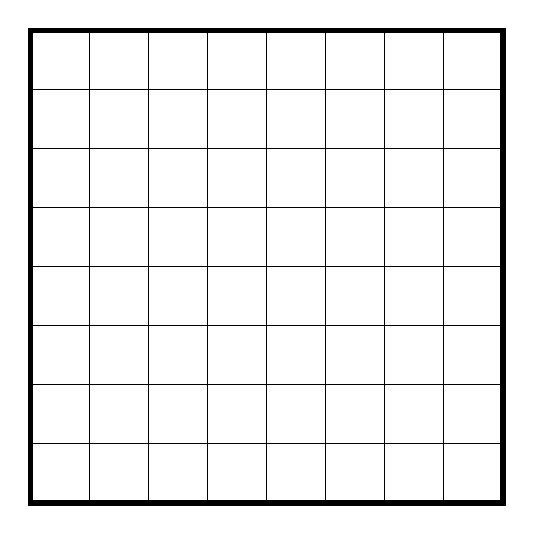
\begin{tikzpicture}[scale=0.75]

\foreach \a in {0,...,8}{
	\draw (\a,0)--(\a,8);
	\draw (0,\a)--(8,\a);
}

\draw[line width = 2] (0,0)--(8,0)--(8,8)--(0,8)--cycle;

\end{tikzpicture} \\ 
And I wonder why this particular shape is so essential: \\
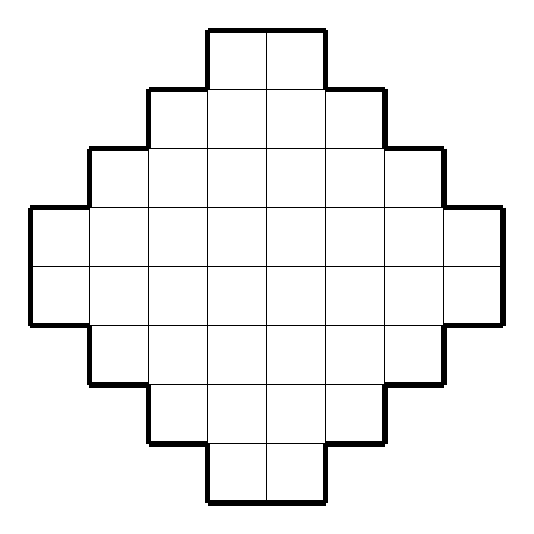
\begin{tikzpicture}[scale=0.75]



\foreach \a in {0,...,3}{

	\draw[line width=2] (\a  ,4-\a)--(\a+1, 4-\a  );
	\draw[line width=2] (\a+1,4-\a)--(\a+1, 4-\a-1);
	
	\draw (   \a, 4-\a)--(   \a, \a-4);
	\draw (-1*\a, 4-\a)--(-1*\a, \a-4);
	
	\draw ( 4-\a,    \a)--(\a-4,    \a);
	\draw ( 4-\a, -1*\a)--(\a-4, -1*\a);

	\def \b {-1}
	\def \c { 1}
		
	\draw[line width=2] (\b*\a  ,\c*4-\c*\a)--(\b*\a+\b*1, \c*4-\c*\a  );
	\draw[line width=2] (\b*\a+\b*1,\c*4-\c*\a)--(\b*\a+\b*1, \c*4-\c*\a-\c*1);
	
	\def \b { 1}
	\def \c {-1}
		
	\draw[line width=2] (\b*\a  ,\c*4-\c*\a)--(\b*\a+\b*1, \c*4-\c*\a  );
	\draw[line width=2] (\b*\a+\b*1,\c*4-\c*\a)--(\b*\a+\b*1, \c*4-\c*\a-\c*1);
	
	\def \b {-1}
	\def \c {-1}
		
	\draw[line width=2] (\b*\a  ,\c*4-\c*\a)--(\b*\a+\b*1, \c*4-\c*\a  );
	\draw[line width=2] (\b*\a+\b*1,\c*4-\c*\a)--(\b*\a+\b*1, \c*4-\c*\a-\c*1);

}

\end{tikzpicture}

\newpage

\noindent Pathetic Tutorial:

\fontfamily{qag}\selectfont \fontsize{12}{10}\selectfont

\begin{verbatim}
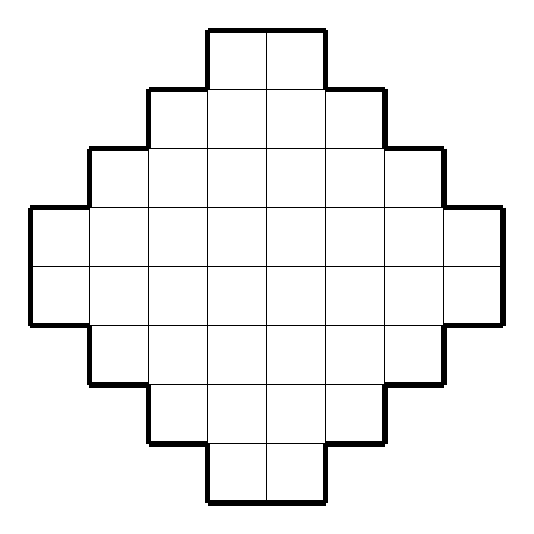
\begin{tikzpicture}[scale=0.75]

\foreach \a in {0,...,3}{

	\draw[line width=2] (\a  ,4-\a)--(\a+1, 4-\a  );
	\draw[line width=2] (\a+1,4-\a)--(\a+1, 4-\a-1);
	
	\draw (   \a, 4-\a)--(   \a, \a-4);
	\draw (-1*\a, 4-\a)--(-1*\a, \a-4);
	
	\draw ( 4-\a,    \a)--(\a-4,    \a);
	\draw ( 4-\a, -1*\a)--(\a-4, -1*\a);

	\def \b {-1}
	\def \c { 1}
		
	\draw[line width=2] (\b*\a     ,\c*4-\c*\a)--(\b*\a+\b*1, \c*4-\c*\a     );
	\draw[line width=2] (\b*\a+\b*1,\c*4-\c*\a)--(\b*\a+\b*1, \c*4-\c*\a-\c*1);
	
	\def \b { 1}
	\def \c {-1}
		
	\draw[line width=2] (\b*\a     ,\c*4-\c*\a)--(\b*\a+\b*1, \c*4-\c*\a     );
	\draw[line width=2] (\b*\a+\b*1,\c*4-\c*\a)--(\b*\a+\b*1, \c*4-\c*\a-\c*1);
	
	\def \b {-1}
	\def \c {-1}
		
	\draw[line width=2] (\b*\a     ,\c*4-\c*\a)--(\b*\a+\b*1, \c*4-\c*\a     );
	\draw[line width=2] (\b*\a+\b*1,\c*4-\c*\a)--(\b*\a+\b*1, \c*4-\c*\a-\c*1);

}

\end{tikzpicture}

\end{verbatim}


\noindent In French the word for tiling is \textit{pavage} -- so literally we are \textbf{paving} the shapes with dominoes. 




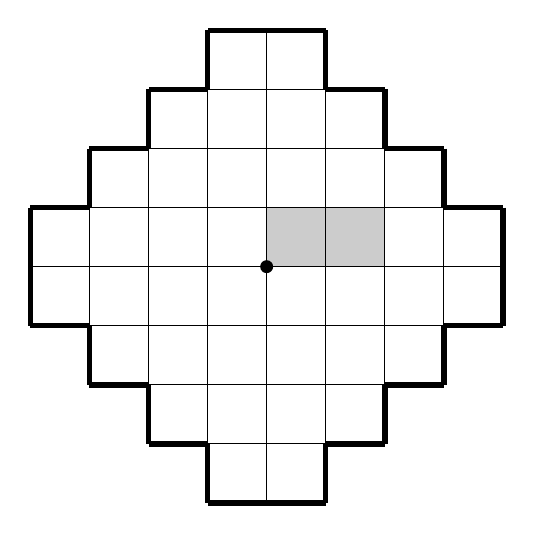
\begin{tikzpicture}[scale=0.75]

\def \b {0}
\def \c {0}


\draw[fill=black!20!white] (\b,\c)--(\b+2,\c)--(\b+2,\c+1)--(\b,\c+1)--cycle;
\draw[fill=black] (\b,\c) circle (0.1);

\foreach \a in {0,...,3}{

	\draw[line width=2] (\a  ,4-\a)--(\a+1, 4-\a  );
	\draw[line width=2] (\a+1,4-\a)--(\a+1, 4-\a-1);
	
	\draw (   \a, 4-\a)--(   \a, \a-4);
	\draw (-1*\a, 4-\a)--(-1*\a, \a-4);
	
	\draw ( 4-\a,    \a)--(\a-4,    \a);
	\draw ( 4-\a, -1*\a)--(\a-4, -1*\a);

	\def \b {-1}
	\def \c { 1}
		
	\draw[line width=2] (\b*\a  ,\c*4-\c*\a)--(\b*\a+\b*1, \c*4-\c*\a  );
	\draw[line width=2] (\b*\a+\b*1,\c*4-\c*\a)--(\b*\a+\b*1, \c*4-\c*\a-\c*1);
	
	\def \b { 1}
	\def \c {-1}
		
	\draw[line width=2] (\b*\a  ,\c*4-\c*\a)--(\b*\a+\b*1, \c*4-\c*\a  );
	\draw[line width=2] (\b*\a+\b*1,\c*4-\c*\a)--(\b*\a+\b*1, \c*4-\c*\a-\c*1);
	
	\def \b {-1}
	\def \c {-1}
		
	\draw[line width=2] (\b*\a  ,\c*4-\c*\a)--(\b*\a+\b*1, \c*4-\c*\a  );
	\draw[line width=2] (\b*\a+\b*1,\c*4-\c*\a)--(\b*\a+\b*1, \c*4-\c*\a-\c*1);

}

\end{tikzpicture}

\newpage

\fontfamily{qag}\selectfont \fontsize{20}{25}\selectfont  


\newpage

\fontfamily{qag}\selectfont \fontsize{12}{10}\selectfont

\begin{thebibliography}{}

\item ...


\end{thebibliography} 

\noindent The most amazing typo ever: \\

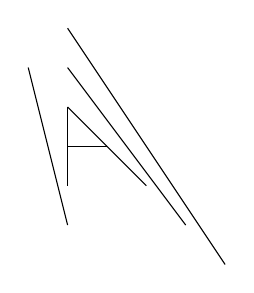
\begin{tikzpicture} [scale=0.5]

\foreach \a in {0,...,5}{
    \draw (\a,5-\a)--(1, \a + 1);
}

\end{tikzpicture}

\begin{verbatim}
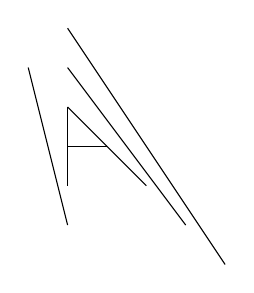
\begin{tikzpicture} [scale=0.5]

\foreach \a in {0,...,5}{

    \draw (\a, 5-\a)--(1, \a + 1);

}

\end{tikzpicture}
\end{verbatim}

\end{document}